\section{Some discussion}

This chapter will concern most of the numerical error analysis and som of the discussion of this analysis as well as an introduction to the methods used for error analysis in general, and how they are adapted to this particular problem.\\


In this numerical setup we will potentially introduce several new error sources in addition to the nomal errors introduced by numerical solution of any equation (see section \ref{some_words_on_PDEs}). 
When a part of the solution acquired is replaced by the solution from another model, which in this case is stochastic, we will change the initial condition to the next iteration in time. 
This might have a number of effects on our final solution. 
When we solve a differential equation numerically we only get an approximation to the actual solution because we are using approximate derivatives (see figure \ref{illustrate_approximate_derivatives}). 
To investigate the error we are introducing we will first need to test that the truncation error of the numerical PDE solver behaves as expected. 
% This can be done by chosing a solution to the PDE, doing a simulation which should yield the same solution and then comparing the two answers. 
% As argued in section \ref{} we will struggle with making the error from the random walk solver be much smaller than $\mathcal{O}(\Delta t)$. 
% We will therefore start by using a simple discretization of the PDE which also has a truncation error of $\mathcal{O}(\Delta t)$. 
% Figure \ref{errorplot_1d} shows the error norm (\ref{}) of only the PDE solver done in 1 dimension plotted for each timestep of the simulation. 
% The manifactured, exact solution is $u(x,t) = \exp\left(-\pi^2t\right)\cos(\pi x)$ and its initial condition is shown in figure \ref{}.

\begin{figure}[H]
 \centering
 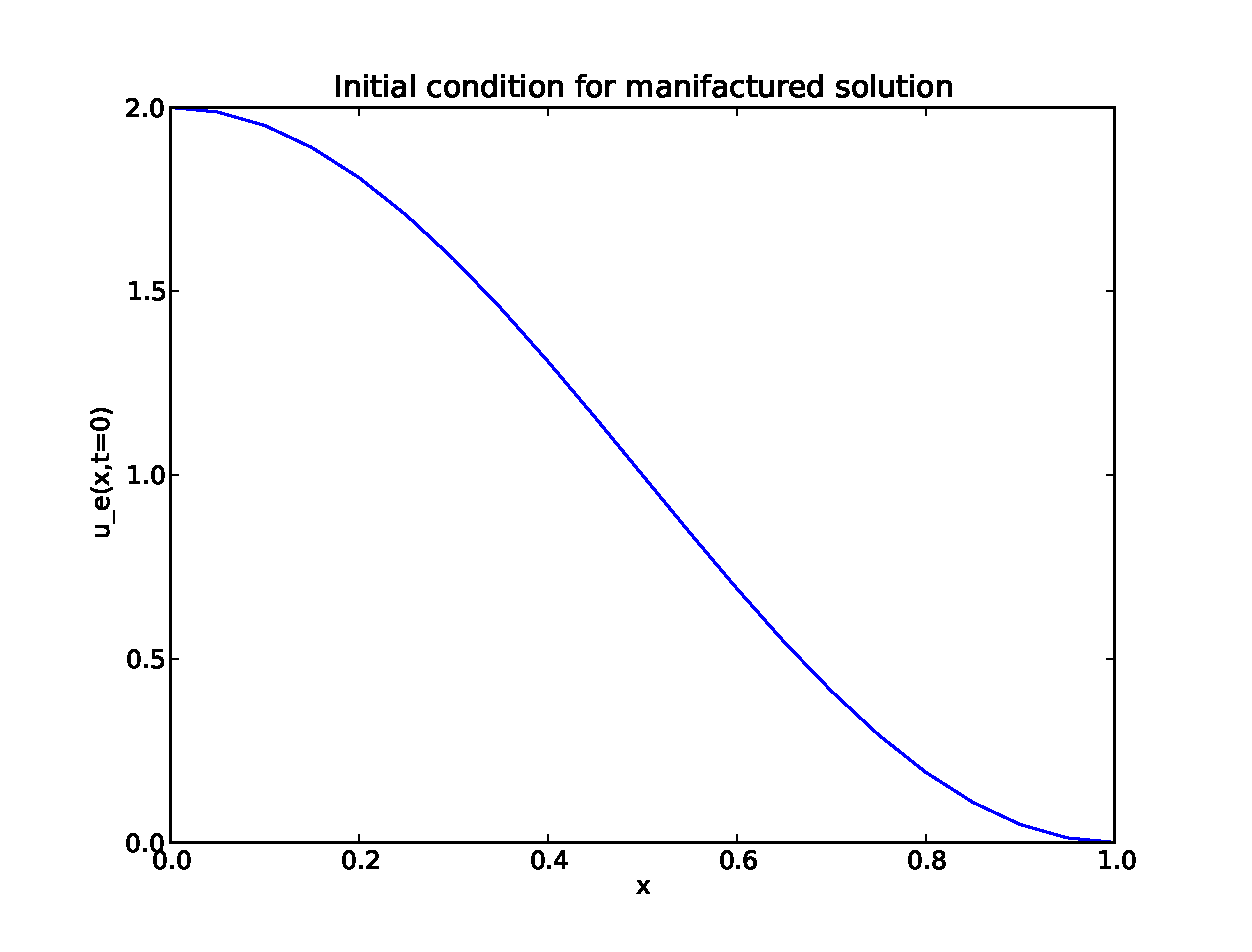
\includegraphics[scale=0.7]{/home/fredriep/Dropbox/uio/thesis/doc/results/experiment_31102013_1017/results/initial_condition.eps}
 \caption[Initial condition in 1d]{Initial condition of manifactured solution in 1d and the simulation.}
 \label{initial_condition_1d}
\end{figure}


\section{Manifactured Solutions}
A normal way of checking that our scheme of choise is implemented correctly is by making an exact solution to the equation and checking that the error is of the expected order. 
As a first, simple implenetation we have worked with the explicit Forward Euler discretization of the simplest form of the diffusion equation \ref{simple_diffusion_equation}. 
This discretization is expected to have an error-term of the order of $\Delta t$, which again is limited by a stability criterion. 
We can now decide that the solution to equation \ref{simple_diffusion_equation} should be
\begin{equation}\label{manifactured_solution_1D}
 u(x,t) = e^{-t\pi^2}\cos(\pi x) +1
\end{equation}
which satisfies our equation if we set the diffusion constant to 1.
\begin{align}
 \frac{\d }{\d t}e^{-t\pi^2}\cos(\pi x) +1 &= D\frac{\d^2}{\d x^2}e^{-t\pi^2}\cos(\pi x) +1\\
 -\pi^2e^{-t\pi^2}\cos(\pi x) &= -\pi^2e^{-t\pi^2}\cos(\pi x) +1 \implies 1 = 1
\end{align}
As we saw in section \ref{truncation_error} the Forward Euler scheme is expected to have an error of the order of $\Delta t$. 
Testing only the scheme first, in 1D we get the following plot \ref{errorplot_FE1D_noWalk} of the maximum of the absolute value of the difference between the exact solution and the numerical solution to the equation. 

\begin{figure}[H]

\centering
\includegraphics[scale=0.7]{/home/fredriep/Dropbox/uio/thesis/doc/results/experiment_31102013_1017/results/deterministic_errorplot.eps}
\caption[Numerical error for 1D Forwar Euler discretization]{Numerical error for 1D Forwar Euler discretization of the PDE. Nothing else is done to the simulation.}
\label{errorplot_FE1D_noWalk}
\end{figure}

We then introduce an area on the domain where we swich models from the normal PDE to an average of the PDE solution and the result of a random walk simulation where the initial condition is the last timestep from the PDE converted to walkers by the conversion rate given in equation \ref{conversion_rate}. In this case we have used the parameters $a=3$, $\Delta t = \frac{\Delta x^2}{3.0}$, $\Delta x = \frac{1}{20}$. 
These parameters makes one unit of $u(x,t)$ equal to some $1000$ walkers. 
\begin{equation}\label{conversion_rate}
 C_{ij} = \frac{a}{\Delta t}U_{ij}
\end{equation}
The area where the model has been replaced is between $x=0.6$ and $x=0.7$, which is three mesh points. 
In the same way as for only the simple 1D PDE case we compare the combined numerical solution from the two models to the exact solution. 
Figure \ref{errorplot_FE1D_Walk_first_attemt} shows that the error is still of the order of $\Delta t$, and the difference between the two models are negligable. 

\begin{figure}[H]
\centering
\includegraphics[scale=0.7]{/home/fredriep/Dropbox/uio/thesis/doc/results/experiment_31102013_1017/results/errorplot.eps}
\caption[Effect of increasing number of walkers]{Numerical error for 1D Forward Euler discretization combined with random walk model between $x=0.6$ and $x=0.7$. Other parameters of importance are $\Delta t\approx 0.00083333$, $\Delta x = 0.05$.}
\label{errorplot_FE1D_Walk_first_attemt}
\end{figure}

As we can se from figure \ref{errorplot_FE1D_Walk_first_attemt} increasing the number of walkers that each ``unit concentration'' corresponds to has a positive effect on the errornorm up to a certain point. 
After we reach $Hc \sim 10^4$ the error is dominated by the truncation error of the Forward Euler scheme. 
This tells us that the error associated with introducing a random walk model on parts of the mesh behaves roughly as we hoped; it tends to zero for large numbers of walkers. 
Meaning of course that the calculations in section \ref{} are not hopeless.



\subsection{The effects of adding drift to the walkers}\label{effect_of_drift_on_walkers}

As shown in section \ref{random_walks_and_drift} adding drift to the walkers will modify our model to represent the convection diffusion equation (\ref{convection_diffusion_equation}) rather than the simple diffusion equation. 
In our analysis so far we have completely ignored the spatial truncation error because it is of second order, and the truncation error in time is of first order. 
When discretizing the convection diffusion equation however, we must take care to use an approximation to the first order spatial derivative that has a truncation error of second order. 
Otherwise the truncation error in this term will completely dominate seeing as $\Delta t<\Delta x$. 
We must also find a new stability criterion for the scheme. \\
As for now, the Leap-frog discretization will do (though it is not by far a perfect choise seeing as it is unstable). 
As a sidenote we can also note that the Neumann boundary condition will be very clear in this scheme. 
$\frac{\d C}{\d n} = 0 \implies \frac{\d C}{\d x} = 0 $ on the boundary, leading to $C_{-1} = C_{1}$ on the boundary and cancelling the drift term on the boundary.
\begin{equation}\label{convection_diffusion_equation_leapfrog}
 C^{n+1} = \frac{D\Delta t}{\Delta x^2}\left(C^n_{i+1}-2C^n_i+C^n_{i-1}\right)-\frac{v\Delta t}{2\Delta x}\left(C^n_{i+1}-C^n_{i-1}\right) + C^n
\end{equation}
The truncation error for the first order derivative using the Leap-frog scheme is obtained as follows
\begin{align*}
 u(t,x+\Delta x) = u(t,x) + \frac{\d u(t,x)}{\d x}\Delta x + \frac{\d^2u(t,x)}{2\d x^2}\Delta x^2 +\mathcal{O}(\Delta x^3)\\
 u(t,x-\Delta x) = u(t,x) - \frac{\d u(t,x)}{\d x}\Delta x + \frac{\d^2u(t,x)}{2\d x^2}\Delta x^2 +\mathcal{O}(\Delta x^3)
\end{align*}
which we recognize as the same error we got from the second order spatial derivatives.\\
If we now do the same analysis as we have already done, by finding a manifactured solution to the convection diffusion equation, implementing a numerical scheme like \ref{convection_diffusion_equation_leapfrog} to solve it after and taking the errornorm. \\
The errornorm does not have to go as $\Delta t$, but it must be halved (approximately) if we halv $\Delta t$. 
Figure \ref{} shows two simulations of equation \ref{convection_diffusion_equation} for $D =1$ and $v=1$ compared to the manifactured solution \ref{manifactured_solution_1D} without adding walkers. 
Before the simulation we must find a source term so the manifactured solution will solve the equation.
\begin{align*}
 -\pi^2\exp\left(-\pi^2t\right)\cos\left(\pi x\right) &= -\pi^2D\exp\left(-\pi^2t\right)\cos\left(\pi x\right) + \pi v \exp\left(-\pi^2t\right)\sin\left(\pi x\right) + f(x,t)\\
 -\pi^2\cos\left(\pi x\right) &= \pi^2D\cos\left(\pi x\right) +\pi v \sin\left(\pi x\right) + \tilde{f}(x) \\
 \tilde{f}(x) &= -\pi\sin\left(\pi x\right)
\end{align*}
Where $f(x,t) = \exp\left(-\pi^2t\right)\tilde{f}(x)$.

\begin{figure}[H]
\centering
\begin{subfigure}[b]{0.48\textwidth}
\includegraphics[width=\textwidth]{/home/fredriep/Dropbox/uio/thesis/doc/results/experiment_05112013_1235/results/deterministic_errorplot.eps}
\caption{}
\label{Verification_convection_diffusion:single_dt}
\end{subfigure}
\begin{subfigure}[b]{0.48\textwidth}
\includegraphics[width=\textwidth]{/home/fredriep/Dropbox/uio/thesis/doc/results/experiment_05112013_1234/results/deterministic_errorplot.eps}
\caption{}
\label{Verification_convection_diffusion:double_dt}
\end{subfigure}
\caption[Verification of Convection diffusion equation implenetation]{Verification of Convection diffusion equation implenetation}
\label{Verification_convection_diffusion}
\end{figure}

As we see from figure \ref{Verification_convection_diffusion} the errornorm is halved when $\Delta t$ is roughly halved, just as we expected. It is also of the order of $\Delta t$, which is nice.  
We can then advance to testing the effect of adding an area of walkers for different values of $Hc$ as before. 
Note that we can no longer use the manifactured solution now if we wish to add drift to the walkers because we have forced the solution to fit the equation by tampering with the source term. 
The effect of
\begin{figure}[H]
\centering
\begin{subfigure}[b]{0.48\textwidth}
\includegraphics[width=\textwidth]{/home/fredriep/Dropbox/uio/thesis/doc/results/experiment_05112013_1237/results/errorplot.eps}
\caption{}
\label{Errortest_convection_diffusion_walkers:few_walkers}
\end{subfigure}
\begin{subfigure}[b]{0.48\textwidth}
\includegraphics[width=\textwidth]{/home/fredriep/Dropbox/uio/thesis/doc/results/experiment_05112013_1239/results/errorplot.eps}
\caption{Adding more walkers still has the desired effect on the error, suggesting that the central limit theorem is at work behind the scenes.}
\label{Errortest_convection_diffusion_walkers:more_walkers}
\end{subfigure}
\caption[Adding walkers influenced by drift]{The figure shows the effect adding walkers influenced by drift has on the error. 
The drift term is the step length, which is quite large. The strangest thig is, however, that changing the direction of the drift has little effect on the error, suggesting that the drift term is completely wrong in relation to the steplength. $\Delta t =8e-5$}
\label{Errortest_convection_diffusion_walkers}
\end{figure}



\subsection{Anisotropic diffusion}

As we discussed in section \ref{random_walks_and_anisotropy} we should also be able to model diffusion where the diffusion constant is not a constant. 
The scheme we derived in section \ref{discretizing} allready takes this into account, and so all we need to do is to add the drift term which was discussed in section \ref{effect_of_drift_on_walkers} to the scheme. 
Like before we should verify that the scheme solves the equation to the expected accuracy by using a manifactured solution \ref{manifactured_solution_1D} and tweaking the source term so this function solved the equation \ref{convection_diffusion_equation}. 
When $v=0$ and $D(x) = \pi x$ the source term becomes
\begin{align*}
 -\pi^2\exp\left(-\pi^2t\right)\cos\left(\pi x\right) &= -\pi\exp\left(-\pi^2t\right)\frac{\d}{\d x}\pi x\sin(\pi x) +f(x,t) \\
 -\pi^2\cos\left(\pi x\right) &= -\pi^2\left(\sin(\pi x) + \pi x\cos(\pi x)\right) +\tilde{f}(x) \\
 \tilde{f}(x) &= \pi^2\left(\sin(\pi x) +\cos(\pi x)(\pi x-1)\right)
\end{align*}
Once again $f(x,t) = \exp\left(-\pi^2t\right)\tilde{f}(x)$. Figure \ref{anisotropic_diffusion_verification} shows the errornorm of the result of simulations of this equation with different values of $\Delta t$.

\begin{figure}[H]
\centering
\begin{subfigure}[b]{0.48\textwidth}
\includegraphics[width=\textwidth]{/home/fredriep/Dropbox/uio/thesis/doc/results/experiment_05112013_1303/results/deterministic_errorplot.eps}
\caption{}
\label{anisotropic_diffusion_verification:single_dt}
\end{subfigure}
\begin{subfigure}[b]{0.48\textwidth}
\includegraphics[width=\textwidth]{/home/fredriep/Dropbox/uio/thesis/doc/results/experiment_05112013_1304/results/deterministic_errorplot.eps}
\caption{}
\label{anisotropic_diffusion_verification:double_dt}
\end{subfigure}
\caption[Verification of anisotropic diffusion equation implenetation]{Verification of anisotropic diffusion equation implenetation}
\label{anisotropic_diffusion_verification}
\end{figure}
Again, the error is of the order of $\Delta t$ and is roughly halved by halving $\Delta t$.
\section{2D}
Doing the same tests is 2D gives slightly different results; adding a 2D walk-domain has an influence on the error, but a rather small one. 
This can, however be tweaked by increasing the conversion parameters.

\begin{equation}
 - \frac{\pi^{2} \operatorname{cos}\left(\pi x\right) \operatorname{cos}\left(\pi y\right)}{e^{\pi^{2} t}}
\end{equation}
\begin{equation}
- \frac{\pi^{2} \left(x + y\right) \operatorname{cos}\left(\pi x\right) \operatorname{cos}\left(\pi y\right)}{e^{\pi^{2} t}} - \frac{\pi \operatorname{sin}\left(\pi x\right) \operatorname{cos}\left(\pi y\right)}{e^{\pi^{2} t}}
\end{equation}
\begin{equation}
- \frac{\pi^{2} \left(x + y\right) \operatorname{cos}\left(\pi x\right) \operatorname{cos}\left(\pi y\right)}{e^{\pi^{2} t}} - \frac{\pi \operatorname{sin}\left(\pi y\right) \operatorname{cos}\left(\pi x\right)}{e^{\pi^{2} t}}
\end{equation}

